% Chapter 3. Three deployment shapes, and what statelessness does to each.
\documentclass[tikz,border=6pt]{standalone}
% Shared look for every TikZ figure in the book.
% Colours match book/preamble.tex exactly. Change both or neither.

\usepackage{tikz}
\usepackage{xcolor}
\usepackage{amsmath}
\IfFileExists{libertinus.sty}{\usepackage[mono=false]{libertinus}}{}
\IfFileExists{inconsolata.sty}{\usepackage[varqu,varl,scaled=0.95]{inconsolata}}{}

\usetikzlibrary{
  arrows.meta, positioning, calc, fit, backgrounds, shapes.geometric,
  shapes.misc, decorations.pathreplacing, decorations.pathmorphing,
  patterns, chains, matrix, shadows.blur
}

\definecolor{ink}{HTML}{15181D}
\definecolor{muted}{HTML}{5B6472}
\definecolor{rule}{HTML}{C9CED6}
\definecolor{wash}{HTML}{F4F5F7}
\definecolor{accent}{HTML}{0F5C8C}
\definecolor{accentsoft}{HTML}{E7F0F6}
\definecolor{warm}{HTML}{B4531A}
\definecolor{warmsoft}{HTML}{FBF0E7}
\definecolor{good}{HTML}{2C6E49}
\definecolor{goodsoft}{HTML}{E9F2EC}
\definecolor{danger}{HTML}{9B2226}
\definecolor{dangersoft}{HTML}{FAECEC}

\tikzset{
  font=\sffamily\small,
  >={Stealth[length=5pt, width=4pt]},
  %
  box/.style={
    draw=rule, line width=0.8pt, fill=wash, rounded corners=2pt,
    inner sep=7pt, align=center, text=ink, minimum height=9mm,
  },
  boxa/.style={box, draw=accent, fill=accentsoft},
  boxg/.style={box, draw=good,   fill=goodsoft},
  boxw/.style={box, draw=warm,   fill=warmsoft},
  boxd/.style={box, draw=danger, fill=dangersoft},
  %
  lane/.style={draw=rule, line width=0.7pt, fill=white, rounded corners=2pt,
               inner sep=6pt, align=center, minimum width=26mm},
  %
  flow/.style={draw=accent, line width=1.0pt, ->},
  flowback/.style={flow, densely dashed},
  flowmuted/.style={draw=muted, line width=0.8pt, ->},
  lifeline/.style={draw=rule, line width=0.7pt, densely dotted},
  %
  lbl/.style={font=\sffamily\scriptsize, text=muted, inner sep=2pt},
  lblink/.style={font=\sffamily\scriptsize, text=ink, inner sep=2pt},
  tag/.style={font=\ttfamily\scriptsize, text=accent, inner sep=2pt,
              fill=white, inner xsep=3pt},
  note/.style={font=\sffamily\scriptsize\itshape, text=muted, align=left},
  %
  band/.style={draw=none, rounded corners=1pt},
  tick/.style={draw=muted, line width=0.6pt},
}

% A horizontal timeline bar segment: \barseg{x0}{x1}{y}{colour}{label}
\newcommand{\barseg}[5]{%
  \fill[#4, rounded corners=1pt] (#1,#3-0.16) rectangle (#2,#3+0.16);
  \node[lbl, text=white, font=\sffamily\scriptsize\bfseries]
       at ({(#1+#2)/2},#3) {#5};
}

\begin{document}
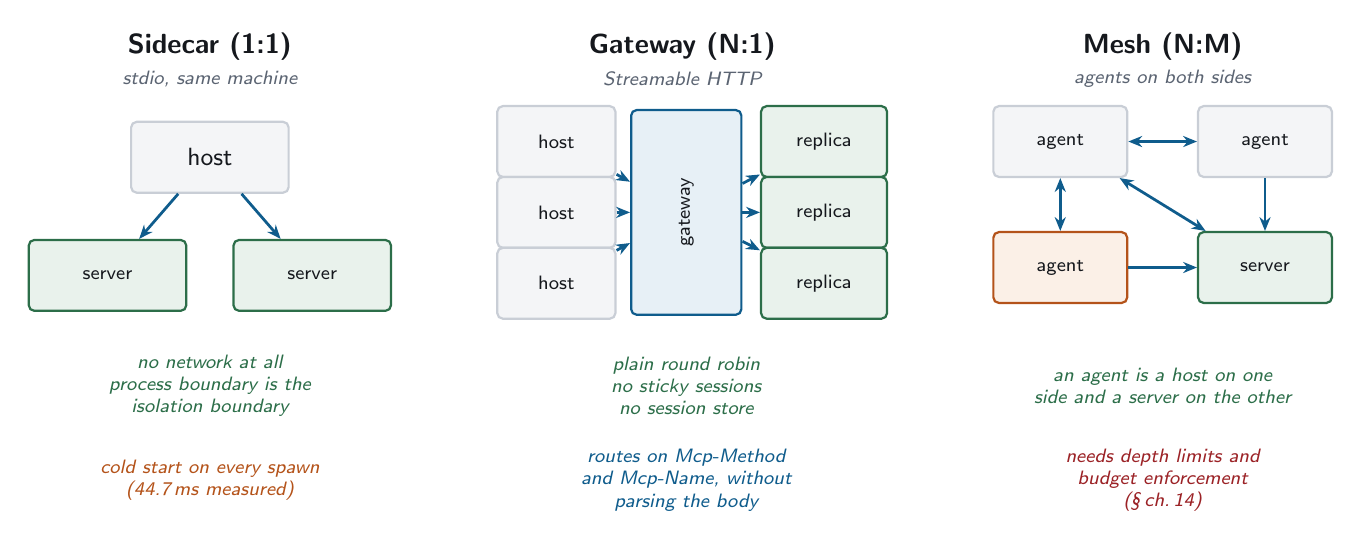
\begin{tikzpicture}[x=1cm, y=1cm]

% ---------------------------------------------------------------- sidecar
\begin{scope}[xshift=0cm]
  \node[lblink, font=\sffamily\bfseries] at (1.5,3.3) {Sidecar (1:1)};
  \node[note, align=center] at (1.5,2.9) {stdio, same machine};

  \node[box, minimum width=20mm] (h) at (1.5,1.9) {host};
  \node[boxg, minimum width=20mm, font=\sffamily\scriptsize] (a) at (0.2,0.4) {server};
  \node[boxg, minimum width=20mm, font=\sffamily\scriptsize] (b) at (2.8,0.4) {server};
  \draw[flow] (h) -- (a);
  \draw[flow] (h) -- (b);

  \node[note, align=center, text=good] at (1.5,-1.0)
    {no network at all\\process boundary is the\\isolation boundary};
  \node[note, align=center, text=warm] at (1.5,-2.2)
    {cold start on every spawn\\(44.7\,ms measured)};
\end{scope}

% ---------------------------------------------------------------- gateway
\begin{scope}[xshift=5.6cm]
  \node[lblink, font=\sffamily\bfseries] at (1.9,3.3) {Gateway (N:1)};
  \node[note, align=center] at (1.9,2.9) {Streamable HTTP};

  \node[box, minimum width=15mm, font=\sffamily\scriptsize] (h1) at (0.3,2.1) {host};
  \node[box, minimum width=15mm, font=\sffamily\scriptsize] (h2) at (0.3,1.2) {host};
  \node[box, minimum width=15mm, font=\sffamily\scriptsize] (h3) at (0.3,0.3) {host};

  \node[boxa, minimum width=14mm, minimum height=26mm, align=center,
        font=\sffamily\scriptsize] (gw) at (1.95,1.2) {\rotatebox{90}{gateway}};

  \node[boxg, minimum width=16mm, font=\sffamily\scriptsize] (r1) at (3.7,2.1) {replica};
  \node[boxg, minimum width=16mm, font=\sffamily\scriptsize] (r2) at (3.7,1.2) {replica};
  \node[boxg, minimum width=16mm, font=\sffamily\scriptsize] (r3) at (3.7,0.3) {replica};

  \foreach \h in {h1,h2,h3} { \draw[flow] (\h) -- (gw); }
  \foreach \r in {r1,r2,r3} { \draw[flow] (gw) -- (\r); }

  \node[note, align=center, text=good] at (1.95,-1.0)
    {plain round robin\\no sticky sessions\\no session store};
  \node[note, align=center, text=accent] at (1.95,-2.2)
    {routes on Mcp-Method\\and Mcp-Name, without\\parsing the body};
\end{scope}

% ------------------------------------------------------------------- mesh
\begin{scope}[xshift=11.9cm]
  \node[lblink, font=\sffamily\bfseries] at (1.7,3.3) {Mesh (N:M)};
  \node[note, align=center] at (1.7,2.9) {agents on both sides};

  \node[box, minimum width=17mm, font=\sffamily\scriptsize] (m1) at (0.4,2.1) {agent};
  \node[box, minimum width=17mm, font=\sffamily\scriptsize] (m2) at (3.0,2.1) {agent};
  \node[boxw, minimum width=17mm, font=\sffamily\scriptsize] (m3) at (0.4,0.5) {agent};
  \node[boxg, minimum width=17mm, font=\sffamily\scriptsize] (m4) at (3.0,0.5) {server};

  \draw[<->, draw=accent, line width=1pt] (m1) -- (m2);
  \draw[<->, draw=accent, line width=1pt] (m1) -- (m3);
  \draw[flow] (m2) -- (m4);
  \draw[flow] (m3) -- (m4);
  \draw[<->, draw=accent, line width=1pt] (m1) -- (m4);

  \node[note, align=center, text=good] at (1.7,-1.0)
    {an agent is a host on one\\side and a server on the other};
  \node[note, align=center, text=danger] at (1.7,-2.2)
    {needs depth limits and\\budget enforcement\\(\S\,ch.\,14)};
\end{scope}

\end{tikzpicture}
\end{document}
